\documentclass[11pt]{article}
\usepackage{../style/forage}
\usepackage{needspace}
% keep headings with the text that follows them
\let\oldsubheading\subheading
\renewcommand{\subheading}[1]{\Needspace{6\baselineskip}\oldsubheading{#1}}
\let\oldheading\heading
\renewcommand{\heading}[1]{\Needspace{8\baselineskip}\oldheading{#1}}

% Figures and tables in figures/ are generated by analysis.ipynb.
% Re-run the notebook if the assumptions change, then recompile.

\newcommand{\product}[4]{% {name}{allocation}{why}{justification}
  \begin{tcolorbox}[enhanced, colback=boxgray, frame hidden, arc=2mm,
      borderline west={1.2mm}{0pt}{navy}, left=5mm, right=4mm, top=2.5mm,
      bottom=2.5mm, breakable]
    {\bfseries\color{navy}#1}\hfill{\small\badge{#2}}\par\smallskip
    \textbf{Why this product:} #3\par\smallskip
    \textbf{Justification:} #4
  \end{tcolorbox}}

\begin{document}

% ================= Title page =================
\begin{titlepage}
  \vspace*{4cm}
  {\color{navy}\fontsize{30}{36}\selectfont Strategic Investment\\[2mm]
  Recommendations}\par\medskip
  {\Large Diversified, Sustainable, Moderate Growth:\\
  A Rebalancing Plan for Summit Investments}\par
  {\color{rulegray}\rule{\linewidth}{0.6pt}}\par\bigskip
  \begin{tabular}{@{}ll}
    \textbf{Client Name:}  & Summit Investments \\
    \textbf{Analyst Name:} & Thiziri Amezza, Sales and Trading Analyst \\
    \textbf{Team:}         & Global Markets Advisory \\
    \textbf{Date:}         & \today \\
  \end{tabular}
  \vfill
  {\small\color{gray}Prepared as part of the Bank of America Global Markets
  Sales and Trading job simulation (Forage). Hypothetical client. Expected
  returns, volatilities and stress shocks are illustrative assumptions; all
  figures and tables are reproducible with \texttt{analysis.ipynb}.}
\end{titlepage}

% ================= Executive summary =================
\heading{Executive Summary}
Summit Investments wants to grow at a moderate pace while becoming more
diversified and more sustainable. Today the portfolio does not reflect those
goals: \textbf{45\% sits in U.S.\ large-cap stocks}, which generate about
\textbf{73\% of the portfolio's total risk}; there is no international or
emerging-market exposure; and there is no green or ESG allocation.

We propose to rebalance in three monthly steps, keeping the overall risk level
unchanged or lower:
\begin{itemize}[leftmargin=1.5em, itemsep=2pt]
  \item \textbf{Diversify:} reduce U.S.\ large-cap stocks from 45\% to 27\%;
  add 6\% \textbf{emerging-market bonds} and 5\% international equities.
  \item \textbf{Mitigate risk:} keep a 22\% core of \textbf{corporate and
  Treasury bonds}, moved to a shorter duration to limit the impact of rising
  rates, and hold 10\% in cash.
  \item \textbf{Invest sustainably:} 7\% \textbf{green ETFs}, a 6\%
  \textbf{ESG mutual fund} and 4\% green bonds --- 17\% in total, above the
  client's 10\% target.
  \item \textbf{Stay stable:} keep 13\% in \textbf{REITs} for long-term
  income.
\end{itemize}

Under our assumptions, the proposed portfolio has a slightly
\textbf{higher expected return (5.9\% vs 5.8\%)} with \textbf{lower volatility
(9.2\% vs 9.4\%)}, the largest single holding falls from 45\% to 27\%, and the
share of risk coming from U.S.\ large-caps drops from 73\% to 43\%.

\infobox{\faClipboardList}{Client at a glance}{
  \item \textbf{Allocation:} Equities 45\% (mostly U.S.\ large-cap), Fixed
  income 30\%, Real estate (REITs) 15\%, Cash 10\%.
  \item \textbf{Priorities:} diversification, risk mitigation,
  sustainability, moderate growth, long-term stability.
  \item \textbf{Targets:} at least 10\% in green ETFs and ESG funds; up to 8\%
  in emerging-market bonds; less reliance on U.S.\ large-caps.
  \item \textbf{Concerns:} rising interest rates, little exposure to
  fast-growing sectors, geopolitical risk in emerging markets.
}

% ================= Client priorities =================
\heading{Client Priorities}

\subheading{Diversification}
The portfolio is concentrated: one asset class (U.S.\ large-cap stocks) is
45\% of the capital and nearly three-quarters of the risk. We address this by
adding new sources of return that behave differently --- emerging-market
bonds, international equities and green assets. The \emph{effective number of
holdings}, a simple measure of how evenly the money is spread, almost doubles
from 3.1 to 6.1.

\subheading{Sustainability}
Sustainability is built into three parts of the portfolio rather than added
as a single position: green ETFs on the equity side, an ESG mutual fund in
the balanced core, and green bonds in fixed income. Together they reach 17\%
of the portfolio, and each is screened for a clear environmental, social and
governance focus, as the client requires.

\subheading{Moderate Growth}
Summit wants consistent returns without excessive volatility. The proposal
adds growth (green ETFs, emerging-market bonds, international equities) but
pays for it by reducing the most concentrated risk, so expected return rises
slightly while expected volatility falls. Return per unit of volatility
improves from 0.62 to~0.64.

% ================= Products =================
\heading{Recommended Financial Products and Justifications}
Each priority is matched with the product best suited to it, using the
Product Alignment Guide.

\product{Product 1: Emerging Market Bonds --- Diversification}{6\%}{%
They give exposure to fast-growing developing economies, and they are
fixed-income securities, so they are less volatile than emerging-market
stocks.}{%
They are the guide's recommended product for diversification and match the
client's stated interest and its target of up to 8\%. We start at 6\% to keep
room below the limit, because geopolitical risk in emerging markets is one of
the client's concerns. A diversified bond fund spreads that risk across many
countries.}

\product{Product 2: Corporate \& Treasury Bonds (shorter duration) --- Risk
Mitigation}{22\%}{%
They provide regular income and stability, and are much less volatile than
equities.}{%
This is the portfolio's anchor in a sell-off: in our equity stress test,
core bonds gain while stocks fall. Rising rates are a client concern, so we
recommend moving to a shorter average duration (about 4 years instead of
about 6). This reduces the price loss when rates rise.}

\product{Product 3: Green ETFs --- Sustainability}{7\%}{%
Low fees, high liquidity and diversified exposure to renewable energy and
clean technology.}{%
They directly answer the client's interest in green ETFs and its concern about
limited exposure to fast-growing sectors such as renewable energy. They are
the most volatile holding, so we keep them at 7\%, which is enough to matter
but small enough to contain the risk.}

\product{Product 4: ESG Mutual Fund --- Moderate Growth}{6\%}{%
An actively managed, balanced fund that invests across asset classes with an
ESG mandate.}{%
It offers steady, professionally managed growth with lower volatility than a
pure equity fund, and it counts towards the sustainability target. With the
green ETFs, it brings the green and ESG fund allocation to 13\%, above the
client's 10\% minimum.}

\product{Product 5: Real Estate Investment Trusts (REITs) --- Long-Term
Stability}{13\%}{%
Real estate exposure without owning property directly, with regular dividend
income and potential capital growth.}{%
REITs provide long-term stability and income. We trim them slightly, from
15\% to 13\%, because higher rates raise property financing costs, but they
remain a core holding.}

\textbf{Supporting positions:} an \textbf{international equities ETF} (5\%)
and \textbf{green bonds} (4\%) complete the plan. They reduce reliance on the
U.S.\ market and extend the sustainability theme into fixed income.

% ================= Proposed actions =================
\heading{Proposed Actions}

\subheading{Reallocate Portfolio Funds}
\begin{center}
  \small\begin{tabular}{@{}lrrr@{}}
\toprule
\textbf{Holding} & \textbf{Current} & \textbf{Proposed} & \textbf{Change} \\
\midrule
US large-cap equities & 45\% & 27\% & \textminus{}18 \\
International equities ETF & 0\% & 5\% & +5 \\
Green ETFs & 0\% & 7\% & +7 \\
ESG mutual fund & 0\% & 6\% & +6 \\
Corporate \& Treasury bonds & 30\% & 22\% & \textminus{}8 \\
Green bonds & 0\% & 4\% & +4 \\
Emerging market bonds & 0\% & 6\% & +6 \\
REITs & 15\% & 13\% & \textminus{}2 \\
Cash & 10\% & 10\% & --- \\
\midrule
\textbf{Total} & 100\% & 100\% & \\
\bottomrule
\end{tabular}\par\smallskip
  {\color{gray}Table 1 --- Current and proposed allocation (\% of
  portfolio).}
\end{center}
The 28 points of new investments are funded by reducing U.S.\ large-cap
stocks (\textminus18), core bonds (\textminus8) and REITs (\textminus2). Cash
stays at 10\% for tactical opportunities and risk management.

\begin{center}
  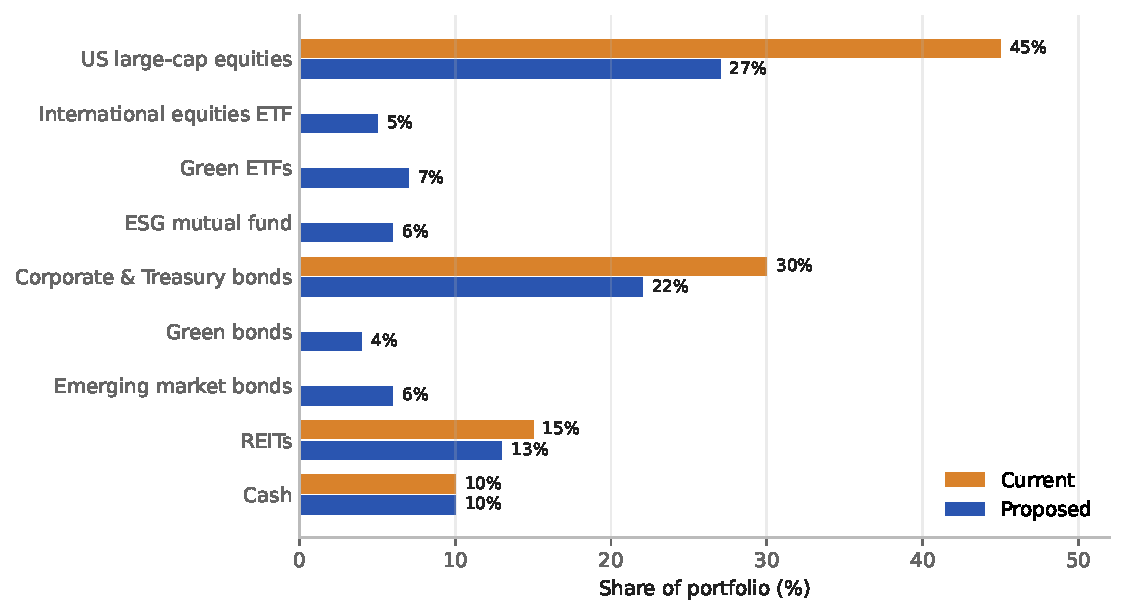
\includegraphics[width=0.9\linewidth]{figures/fig1_allocation.pdf}\par
  {\small\color{gray}Figure 1 --- Current vs.\ proposed allocation.}
\end{center}

\subheading{Introduce New Investments}
To avoid investing everything at a single market level, we implement the plan
in three monthly steps:
\begin{enumerate}[leftmargin=1.5em, itemsep=2pt]
  \item \textbf{Month 1 --- Sustainability:} buy green ETFs (7\%), the ESG
  mutual fund (6\%) and green bonds (4\%), funded by reducing U.S.\ large-cap
  stocks.
  \item \textbf{Month 2 --- Diversification:} buy the international equities
  ETF (5\%) and the first half of the emerging-market bonds (3\%). Shorten
  the duration of the core bond portfolio.
  \item \textbf{Month 3 --- Complete:} after reviewing emerging-market
  conditions, add the remaining 3\% of emerging-market bonds and trim REITs
  to 13\%.
\end{enumerate}

\subheading{Monitor Performance}
\begin{itemize}[leftmargin=1.5em, itemsep=2pt]
  \item \textbf{Monthly:} a short dashboard of performance, volatility and
  allocation drift.
  \item \textbf{Quarterly:} a review meeting. Rebalance any holding that
  drifts more than 2 points from its target.
  \item \textbf{Triggers:} keep emerging-market bonds below the 8\% ceiling,
  and reduce them to 4\% if geopolitical risk rises sharply. Review bond
  duration whenever the interest-rate outlook changes.
  \item \textbf{Annually:} check that the ESG funds still meet Summit's
  sustainability criteria.
\end{itemize}

% ================= Expected outcomes =================
\heading{Expected Outcomes}
\begin{center}
  \small\begin{tabular}{@{}lrr@{}}
\toprule
\textbf{Metric} & \textbf{Current} & \textbf{Proposed} \\
\midrule
Expected annual return$^{\dagger}$ & 5.82\% & 5.92\% \\
Expected volatility$^{\dagger}$ & 9.4\% & 9.2\% \\
Return per unit of volatility & 0.62 & 0.64 \\
Largest single holding & 45\% & 27\% \\
Effective number of holdings & 3.1 & 6.1 \\
US large-cap share of total risk & 73\% & 43\% \\
International \& emerging-market exposure & 0\% & 11\% \\
Sustainable exposure (green ETFs, ESG, green bonds) & 0\% & 17\% \\
\bottomrule
\end{tabular}\par\smallskip
  {\color{gray}Table 2 --- Portfolio metrics. $^{\dagger}$Based on illustrative
  long-run assumptions for each asset class (see Appendix); not a forecast.}
\end{center}

\begin{center}
  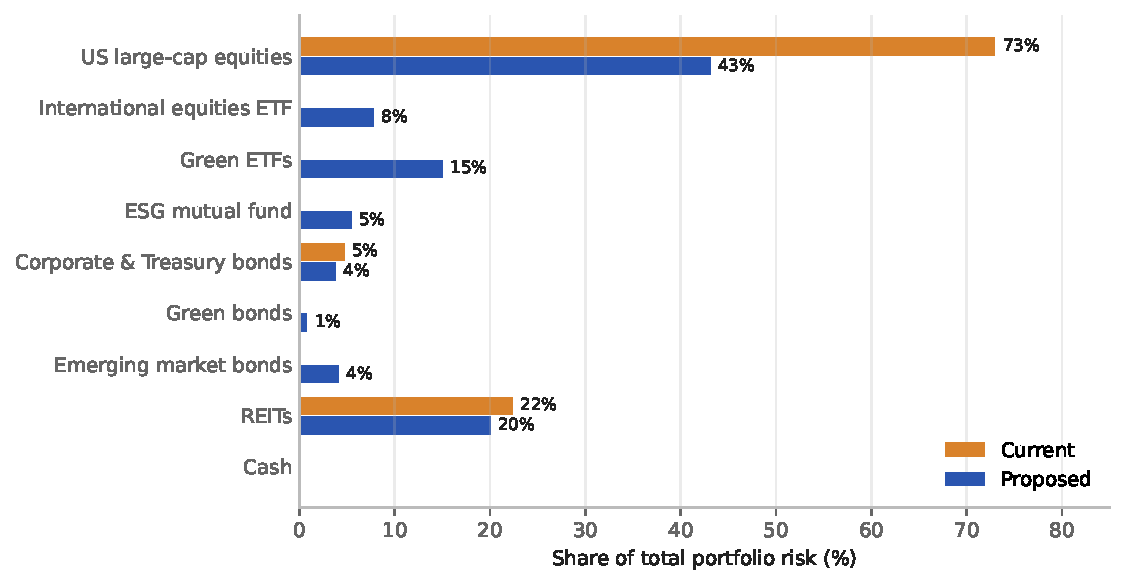
\includegraphics[width=0.9\linewidth]{figures/fig2_risk_contribution.pdf}\par
  {\small\color{gray}Figure 2 --- Share of total portfolio risk contributed by
  each holding.}
\end{center}

\begin{itemize}[leftmargin=1.5em, itemsep=3pt]
  \item \textbf{Better diversification:} U.S.\ large-caps go from 73\% to
  43\% of total risk; 11\% is invested internationally (previously none).
  \item \textbf{Sustainability built in:} 17\% in green ETFs, ESG funds and
  green bonds (previously none).
  \item \textbf{Moderate growth with no extra risk:} expected return rises
  slightly while expected volatility falls.
\end{itemize}

\subheading{Stress Tests: the Client's Three Concerns}
\begin{center}
  \begin{minipage}{\linewidth}\centering
  \small\begin{tabular}{@{}lrrr@{}}
\toprule
\textbf{Scenario} & \textbf{Current} & \textbf{Proposed} & \textbf{Difference} \\
\midrule
Rates +1 pt & \textminus{}4.80\% & \textminus{}4.54\% & +0.26 pts \\
Equity sell-off & \textminus{}10.65\% & \textminus{}10.75\% & \textminus{}0.10 pts \\
Emerging-market crisis & \textminus{}1.35\% & \textminus{}2.16\% & \textminus{}0.81 pts \\
\bottomrule
\end{tabular}\par\smallskip
  {\color{gray}Table 3 --- Immediate portfolio impact of each scenario
  (illustrative shocks; see Appendix).}
  \end{minipage}
\end{center}
\begin{center}
  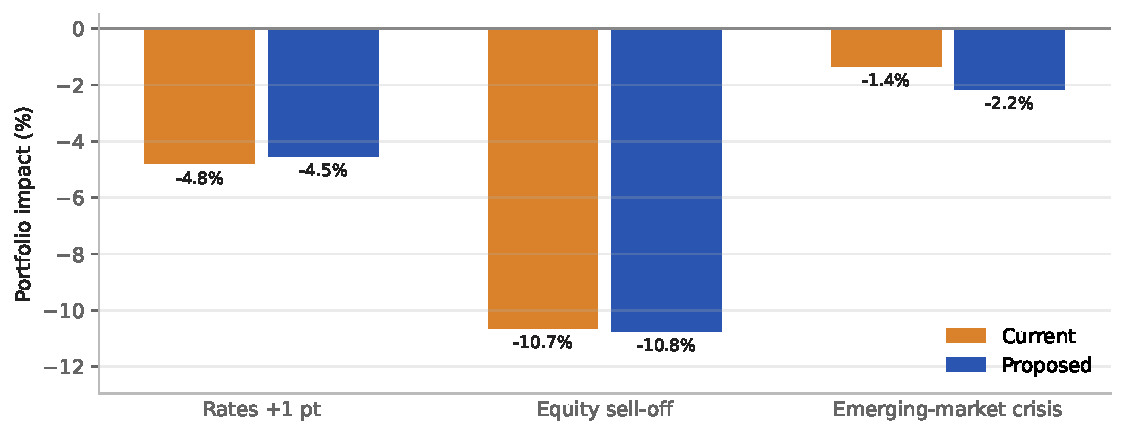
\includegraphics[width=0.9\linewidth]{figures/fig3_stress.pdf}\par
  {\small\color{gray}Figure 3 --- Stress-test results.}
\end{center}
\begin{itemize}[leftmargin=1.5em, itemsep=3pt]
  \item \textbf{Rising rates:} the proposal loses less (\textminus4.5\% vs
  \textminus4.8\%), mainly because of the shorter bond duration.
  \item \textbf{Equity sell-off:} the impact is about the same (\textminus10.8\%
  vs \textminus10.7\%). The new growth holdings are offset by the balanced
  ESG fund and the bonds.
  \item \textbf{Emerging-market crisis:} the proposal loses more
  (\textminus2.2\% vs \textminus1.4\%). This is the cost of diversifying into
  emerging markets, which is why that allocation is capped at 6\%, phased in
  and backed by a reduction trigger.
\end{itemize}

% ================= Conclusion =================
\heading{Conclusion}
This plan aligns Summit Investments' portfolio with its priorities. It
diversifies away from a heavy reliance on U.S.\ large-caps, makes
sustainability a core part of the portfolio, and targets moderate growth
without increasing overall risk. Every change uses established, liquid
products, is introduced gradually, and comes with clear monitoring rules and
triggers.

We would welcome the opportunity to discuss these recommendations with your
team and agree on an implementation timeline. Please let us know a convenient
time for a follow-up meeting, or reach out with any questions in the meantime.

% ================= Appendix =================
\newpage
\heading{Appendix --- Methodology and Assumptions}
\begin{itemize}[leftmargin=1.5em, itemsep=3pt]
  \item \textbf{Data:} weights, targets and concerns come from the Client
  Profile Reference Sheet; product characteristics from the Product Alignment
  Guide.
  \item \textbf{Capital market assumptions (annual):} expected return /
  volatility of 7.0\% / 16\% for U.S.\ and international equities, 8.5\% / 24\%
  for green ETFs, 5.5\% / 10\% for the ESG balanced fund, 4.5\% / 5--6\% for
  core and green bonds, 6.5\% / 10\% for emerging-market bonds, 6.5\% / 18\% for
  REITs, and 3.5\% / 0.5\% for cash. Correlations are set by asset-class group
  (for example, 0.80 between equity holdings and 0.10 between equities and
  core bonds).
  \item \textbf{Metrics:} portfolio volatility $\sigma_p=\sqrt{w^\top\Sigma
  w}$. The risk contribution of holding $i$ is $w_i(\Sigma w)_i/w^\top\Sigma
  w$. The effective number of holdings is $1/\sum_i w_i^2$.
  \item \textbf{Stress shocks:} \emph{Rates +1 pt} --- bonds \textminus4\% to
  \textminus6\% depending on duration, REITs and green ETFs \textminus8\%.
  \emph{Equity sell-off} --- equities \textminus20\%, green ETFs \textminus28\%,
  REITs \textminus15\%, core bonds +2\%. \emph{Emerging-market crisis} ---
  emerging-market bonds \textminus12\%, international equities
  \textminus6\%.
  \item \textbf{Limits:} the assumptions are illustrative and not a forecast.
  They are kept in one place in \texttt{analysis.ipynb} so that they can be
  replaced by the desk's own figures and the analysis re-run.
\end{itemize}
\end{document}
